\TFRGB{voir page}{see page} \pageref{alea}


\begin{tabular}{|c|c|} \hline  

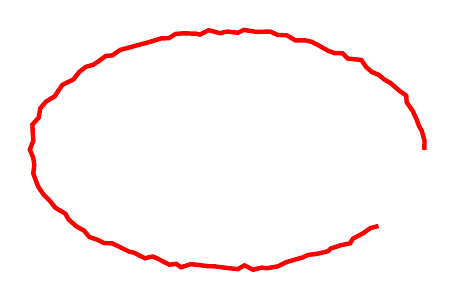
\begin{tikzpicture}[baseline=0pt]
\draw [decorate,blue,ultra thick,red,decoration={random steps,amplitude=1pt,segment length=3pt}]
(0,0)  arc (0:320:2.5 and 1.5);
\end{tikzpicture}
&  
\parbox{8cm}{ 
\BS{draw}[decorate,decoration=\AC {random steps, amplitude=1pt,segment length=3pt}]  (0,0)  arc (0:320:2.5 and 1.5);}
\\ \hline
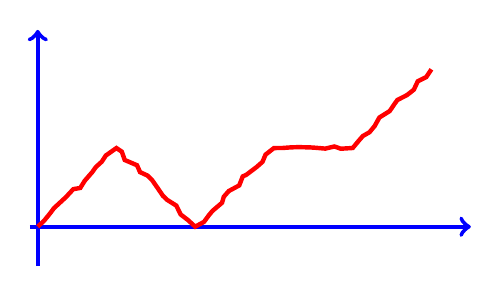
\begin{tikzpicture}[baseline=0pt]
\draw[->,blue,ultra thick] (-.1,0) -- (5.5,0);
\draw[->,blue,ultra thick] (0,-0.5) -- (0,2.5);
 \draw[decorate,blue,ultra thick,red,decoration={random steps,amplitude=1pt,segment length=3pt}] plot coordinates {(0,0) (1,1) (2,0) (3,1) (4,1) (5,2)};
\end{tikzpicture}
&  
\parbox{8cm}{ 
\BS{draw}[decorate,decoration=\AC {random steps, amplitude=1pt,segment length=3pt}] plot coordinates {(0,0) (1,1) (2,0) (3,1) (4,1) (5,2)};}
\\ \hline  
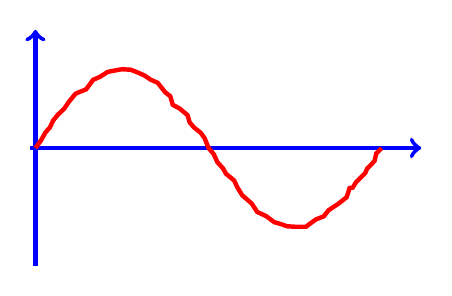
\begin{tikzpicture}[domain=0:6.28,ultra thick,x=0.7cm,baseline=0pt]
%\draw[very thin,color=gray] (-0.1,-2.1) grid (4.1,2.1);
\draw[->,blue,ultra thick] (-.1,0) -- (7,0);
\draw[->,blue,ultra thick] (0,-1.5) -- (0,1.5);
\draw[decorate,red,decoration={random steps,amplitude=1pt,segment length=3pt}] plot  (\x,{sin(\x r)});
\end{tikzpicture}
&
\parbox{8cm}{ 
\BS{draw}[decorate, decoration=\AC{random steps, amplitude=1pt,segment length=3pt}] plot  (\BS{x},{sin(\BS{x} r)});} 
\\ \hline 
\end{tabular} 


